% -*- fill-column: 85; -*-
%!TEX root = ../dissertation.tex

\section{Introduction}
\label{s:intro}

Applications are migrating to the cloud
in search of scalability, resilience, and cost-efficiency. At the same
time, silicon scaling has stalled, precipitating a wave
of new specialized hardware accelerators such as TPUs~\cite{jouppi2016google} and IPUs~\cite{graphcore},
%and streaming accelerators~\cite{QAT} to complement already common
and on-demand GPU and FPGA support from cloud providers.
Accelerators have driven the success of emerging application domains in the cloud~\cite{mlmovetocloud, genomicscloud},
%%, like machine
%%learning} and genomics~\cite{genomicscloud},
but cloud computing and hardware specialization are on a collision course.
Cloud applications run on virtual infrastructure, %
but practical virtualization support for accelerators has yet to arrive.
Cloud providers routinely support accelerators~\cite{amazon_ec2,google-gpu,google-cmle,gpucloud,amazon_f1,olympus},
but do so using PCIe pass-through techniques that dedicate physical hardware to VMs,
despite the wealth of techniques known in the literature~\cite{vCUDA, gVirt,suzuki2014gpuvm, svga, duato2009efficient, rCUDA, gVirtuS, gupta2009gvim, gottschlag2013logv, kvmgt, vfpgamanager, waldspurger-iovirt, li2011gpu, vasila-gvm16, vmCUDA, yeh2017pagoda,trillium}.
This sacrifices the consolidation that drives their business, and leads inevitably to
hardware under-utilization~\cite{simultaneous_multikernel,improving_gpu,gpl,fiddle}.


\begin{figure}[!htp]
	\centering
	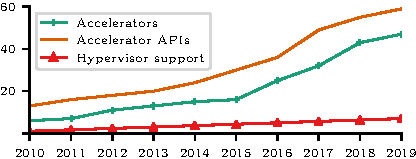
\includegraphics[width=\linewidth]{ava/data/technology_trend/technology_trend.pdf}%
	\caption{The number of accelerators (discrete GPUs and AI
      accelerators) and APIs released since 2010 compared to the number of accelerators officially supported by production hypervisors (VMware ESX, Citrix XenServer, and Microsoft Hyper-V).
      % \ref{l:api_revisions} API major revisions; \ref{l:accelerator_arch} accelerator architectures; \ref{l:hypervisor_arch_support} accelerator architectures supported by hypervisors.
      This data was drawn from release notes and specification sheets.
      % TODO: \amp{This figure has been squished vertically. Regenerate with new aspect-ratio so as to avoid ugly squished text.}
  %\reviewer{F}{I don't think Fig 1 is of much use, your work is a case in point: A single automated approach can deal with many architectures and API revisions, so what is to be read from this?}
  %\cjr{F is pointing out our contribution, but somehow missing it. Dispatched by adding a bullet to the contribution list that claims exactly this.}
  }
	\label{fig:trends}
\end{figure}

The problem is increasingly urgent, as hypervisors have not kept pace with accelerator innovation.
Figure~\ref{fig:trends} shows the evolution of accelerator framework APIs, accelerator architectures, and hypervisor
support for them over the last decade. Specialized hardware and frameworks
emerge far faster than hypervisors support them and the gap is widening.
Many factors contribute to this trend, but lack of demand is \emph{not} among them,
evinced by the wide variety of accelerators currently available from cloud providers~\cite{amazon_ec2,google-gpu,google-cmle,gpucloud,amazon_f1,olympus,cloud-tpu}.
The challenge is technical: hypervisor-level accelerator virtualization requires substantial engineering effort and the design space features multiple
fundamental trade-offs for which a ``sweet spot'' has remained elusive.
%~\cjr{We can do better than this, but at least it actually expresses the real problem. Iterate.}

Practical virtualization must support sharing and isolation under flexible policy
with minimal overhead. The structure of current accelerator stacks makes this
combination extremely difficult to achieve.
Accelerator stacks are \emph{silos} (Figure~\ref{fig:silo})
comprising proprietary layers communicating through memory mapped interfaces.
This opaque organization makes it \emph{impractical} to interpose intermediate layers
to form an efficient and compatible virtualization boundary (\S\ref{s:properties}).
The remaining interposable interfaces leave designers with untenable alternatives
that sacrifice critical virtualization properties such as interposition and compatibility (\S\ref{s:bg_tech}).

This paper describes \Model, which addresses the fundamental limitations of existing accelerator virtualization techniques.
\Model combines API-agnostic para-virtual stack components with a DSL (Domain-Specific Language) and a compiler to automate construction and deployment of guest libraries, hypervisor-level resource management, and \workers.
\Model uses an abstract para-virtual device
to serve as a transport endpoint for forwarding the public APIs of vendor-provided frameworks
(e.g. CUDA or TensorFlow).
Unlike currently popular user-space API remoting solutions~\cite{bitfusion,xaas,vmCUDA,rCUDA,cu2rcu},
% which compromise hypervisor-level resource management and strong isolation,
\model preserves hypervisor-level resource management and strong isolation
using a novel technique called
\emph{\noveltechnique (\novtechabbrv)}.
\novtechabbrv forwards API calls over hypervisor-managed communication channels,
inserting au\-to\-ma\-tically-generated resource management components at the transport layer
to enforce policies from the DSL specification.
Critically, \emph{automation} from \Model enables hypervisors to keep up with fast accelerator evolution: automatic generation of
components dramatically shortens the development cycle.
As Figure~\ref{fig:trends} suggests, a solution that tracks API framework evolution can track hardware evolution as well.

\Model supports a broad range of currently-shipping
compute offload accelerators.
We virtualized \numaccelerators accelerators including NVIDIA and AMD GPUs,
Google TPUs, and Intel QuickAssist.
Virtualizing an API framework using \model requires modest developer effort:
a single developer virtualized OpenCL in a handful of days,
a stark contrast to the person-years of developer effort for
VMware's SVGA II~\cite{svga} or BitFusion's FlexDirect~\cite{bitfusion}.
\Model provides
near-native performance (e.g., 2.4\% slowdown for TensorFlow and 5.6\% for CUDA),
% \hyu{TODO: just leave CUDA, or specify that this TF is the handwritten one.}
%, and 7\% slowdown for NVIDIA OpenCL excluding outliers in Figure~\ref{fig:end2end}),
enforces isolation and fair sharing (\S\ref{s:properties}) across guests,
and supports live migration.
\Model is available at GitHub \mbox{\href{https://github.com/utcs-scea/ava}{utcs-scea/ava}}.
We make the following contributions:

\begin{itemize}[nosep,leftmargin=1em,labelwidth=*,align=left]
\item We demonstrate feasibility of automatically constructed virtual accelerator support, using a single technique to support many architectures, APIs, versions, and policies.
\item We introduce \noveltechnique (\novtechabbrv) to enable
hypervisor-enforced isolation and sharing policies unachievable with current
SR-IOV and API remoting systems (\S\ref{s:motivation}).
\item We describe a novel DSL, \speclang, for describing API functions, resources, and policies to enable automatic construction of virtual stacks starting from native API header files.
\item We evaluate \model on \numaccelerators accelerators showing low effort, strong properties, and good performance (\S\ref{s:eval}).
%\item We identify fundamental challenges in the accelerator virtualization design space (\S\ref{s:background}).
\end{itemize}
